% 第12章第5节：构造策略（消元次序的选择、弦图与完美消元序、完美消元序的构造与核验、团树的构造、构建结果的检验）。

\section{构造策略}
\label{sec:graph-tree-decomposition-construction}

前几节说明了消元次序与树分解怎样互相转换，但没有说明怎样得到规模小的结构。本节在已经建立的等价关系上讨论实际构造：用局部规则选择消元次序；在弦图上利用不需补边的完美消元序；把弦图的极大团借第~\ref{chap:minimum-spanning-tree}章的最大权生成树连成团树；最后逐项检验构建结果。本节的算法只做结构操作，输出袋和袋之间的连接，不计算数值表；输出中实际的袋大小是第~\ref{sec:graph-dp-computation-cost}节代价分析的输入。

\subsection{消元次序的选择}
\label{sec:graph-dp-order-heuristics}
\label{sec:graph-dp-elimination-orders}

\subsubsection{次序对消元簇的影响}

由定理~\ref{thm:graph-dp-elimination-decomposition}，任何消元次序都给出合法的结构，但不同次序产生的消元簇可以相差很多。在三元作用域例子上比较两种次序：$(1,4,2,3)$与先消$x_2$的$(2,1,3,4)$。前者每一步被消去的顶点的邻居都已两两相邻，不产生填充边，消元簇依次为$\{1,2,3\},\{2,3,4\},\{2,3\},\{3\}$。后者第一步要处理$\{1,2,3,4\}$并补入$\{1,4\}$，此后的消元簇为$\{1,3,4\},\{3,4\},\{4\}$。表~\ref{tab:graph-dp-elimination-orders}列出了两种次序每一步的作用域和规模，图~\ref{fig:graph-dp-elimination-orders}画出了对应的图变化。

\begin{table}[!htb]
  \centering
  \caption{三元作用域例子上两种消元次序的逐步规模。“枚举”指计算新函数时要比较的候选组合数，即消元簇上的配置数；“输出”指新函数表的项数，回溯表的项数与之相同。}
  \label{tab:graph-dp-elimination-orders}
  \begin{tabular}{cccccccc}
    \toprule
    \multicolumn{4}{c}{次序$(1,4,2,3)$} & \multicolumn{4}{c}{次序$(2,1,3,4)$}\\
    \cmidrule(lr){1-4}\cmidrule(lr){5-8}
    消去 & 新作用域 & 枚举 & 输出 & 消去 & 新作用域 & 枚举 & 输出\\
    \midrule
    $x_1$ & $\{2,3\}$ & $8$ & $4$ & $x_2$ & $\{1,3,4\}$ & $16$ & $8$\\
    $x_4$ & $\{2,3\}$ & $8$ & $4$ & $x_1$ & $\{3,4\}$ & $8$ & $4$\\
    $x_2$ & $\{3\}$ & $4$ & $2$ & $x_3$ & $\{4\}$ & $4$ & $2$\\
    $x_3$ & $\varnothing$ & $2$ & $1$ & $x_4$ & $\varnothing$ & $2$ & $1$\\
    \midrule
    合计 & & $22$ & $11$ & 合计 & & $30$ & $15$\\
    \bottomrule
  \end{tabular}
\end{table}

\begin{figure}[!htb]
  \centering
  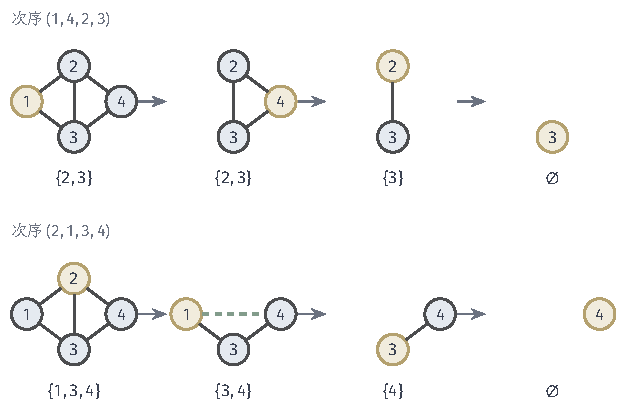
\includegraphics[width=105.004mm]{figures/01-basic-mathematics/04-graphs/tikz/c5-elimination-orders/figure.pdf}
  \caption{两种消元次序下原始图的变化。上行按$(1,4,2,3)$消元，每一步被消去的黄色顶点的邻居都已两两相邻，不产生填充边，新函数至多读取两个变量。下行按$(2,1,3,4)$消元，消去$2$时要补入填充边$\{1,4\}$（第二个图中的绿色虚线），新函数读取三个变量。每个图下方标出消去黄色顶点后新函数的作用域。}
  \label{fig:graph-dp-elimination-orders}
\end{figure}

第一种次序的最大中间表只有$4$项，第二种有$8$项。在这个小例子里差别不大；但若每个变量有$q$个状态，读取$r$个变量的表就有$q^r$项，多读取一个变量意味着表扩大$q$倍。

次序选得不好时，即使在树上也会产生大表：在第~\ref{sec:graph-dp-tree-messages}小节的分叉树上先消去中心$3$，它的邻居$1,2,4$两两补边，新函数要读取三个变量；而按后序消元时不产生任何填充边。两种次序算出的最小值相同（第~\ref{sec:graph-dp-min-cost-correctness}小节），差别只在中间表的规模。

\subsubsection{贪心规则}

定理~\ref{thm:graph-dp-treewidth-induced-width}把找好的树分解归结为找诱导宽度小的消元次序。在一般图上找诱导宽度最小的次序是困难的组合问题，实践中常用局部规则逐轮挑选顶点，得到一个可用但不保证最优的次序。

消去一个顶点，就是把它的全部当前邻居拉进同一个袋，并让它们两两相邻。代价因此体现在两处：它的当前邻居越多，这一步的袋越大；邻居之间缺的边越多，要补的填充边越多，剩下的图越稠密，以后的袋也可能越大。据此有两条常见规则：\term{最小度启发式}（min-degree），选当前邻居最少的顶点；\term{最小填充启发式}（min-fill），选消去时需要补边最少的顶点，即当前邻域中缺少的边数最少者。两条规则都只看当前这一步。

\paragraph{算法实现}

原图和评分规则在运行中不变。算法维护三项状态：
\begin{itemize}
  \item 当前图：初值为原图的副本；
  \item 已输出的次序：初值为空；
  \item 各轮的袋和填充边：初值为空。
\end{itemize}
每一轮依次做三件事：
\begin{itemize}
  \item 评分：在当前图上为每个剩余顶点计算评分，即当前度数或当前缺边数；
  \item 选择：取评分最小者，评分相同时取编号最小者，记为$v$；
  \item 消去：记录袋$\{v\}\cup N(v)$，其中$N(v)$是$v$的当前邻居，把$N(v)$补成团并记录填充边，删去$v$，把$v$追加到次序末尾。
\end{itemize}
当前图为空时停止。

\begin{algorithm}[贪心选择消元次序]
\label{alg:graph-dp-greedy-order}
输入：非空有限无向图和一条评分规则（当前度数或当前缺边数）。输出：消元次序、各轮的袋和填充边。
\begin{enumerate}
  \item 对当前图中的每个顶点按规则计算评分，取评分最小者，评分相同时取编号最小者，记为$v$。
  \item 记录袋$\{v\}\cup N(v)$，把$N(v)$补成团，删去$v$，并把$v$追加到次序末尾。
  \item 若图非空，回到第1步，并在更新后的图上重新计算评分。
\end{enumerate}
\end{algorithm}

评分必须在每轮更新后的图上重算。若只按初始度数排一次序，或用原图的缺边数代替当前缺边数，得到的就不是这两条规则，因为补边会改变其他顶点的度数和邻域。

\paragraph{执行过程}
图~\ref{fig:graph-dp-min-degree-min-fill}的图有六个顶点和边$\{1,3\},\allowbreak\{1,4\},\allowbreak\{1,5\},\allowbreak\{1,6\},\allowbreak\{2,3\},\allowbreak\{2,4\},\allowbreak\{2,6\},\allowbreak\{3,5\},\allowbreak\{4,5\},\allowbreak\{5,6\}$。初始度数依次为$4,3,3,3,4,3$；缺边数依次为$3,3,2,2,3,2$，例如顶点$2$的邻居$3,4,6$两两不相邻，缺$3$条边，而顶点$3$的邻居$1,2,5$中只缺$\{1,2\}$与$\{2,5\}$。表~\ref{tab:graph-dp-greedy-order-trace}并列两条规则的各轮结果。

最小度规则的执行如下：
\begin{itemize}
  \item 第$1$轮：度数为$3$的有$2,3,4,6$，按编号选$2$，袋为$\{2,3,4,6\}$，补入$\{3,4\},\allowbreak\{3,6\},\allowbreak\{4,6\}$。
  \item 第$2$轮：剩下的五个顶点因此两两相邻，度数都是$4$，按编号选$1$，袋为$\{1,3,4,5,6\}$，宽度升到$4$。
  \item 第$3$至$6$轮：剩余图始终是完全图，依次选$3,4,5,6$，不再补边。
\end{itemize}
最小填充规则的执行如下：
\begin{itemize}
  \item 第$1$轮：缺边数为$2$的有$3,4,6$，按编号选$3$，袋为$\{1,2,3,5\}$，补入$\{1,2\}$与$\{2,5\}$。
  \item 第$2$轮：$4$的邻居$1,2,5$已两两相邻，缺边数为$0$；$6$的缺边数也是$0$，按编号选$4$，袋为$\{1,2,4,5\}$。
  \item 第$3$至$6$轮：剩下的四个顶点两两相邻，依次选$1,2,5,6$，不再补边。
\end{itemize}
最大袋含$4$个顶点，宽度为$3$，比最小度规则少$1$。

\begin{table}[!htb]
  \centering
  \caption{两条贪心规则在图~\ref{fig:graph-dp-min-degree-min-fill}的六顶点图上的各轮结果。“选中”列括号内是该顶点当轮的评分（最小度规则为当前度数，最小填充规则为当前缺边数），“补边”列是该轮补入的填充边条数。}
  \label{tab:graph-dp-greedy-order-trace}
  \small
  \begin{tabular}{@{}ccccccc@{}}
    \toprule
    & \multicolumn{3}{c}{最小度} & \multicolumn{3}{c}{最小填充}\\
    \cmidrule(lr){2-4}\cmidrule(lr){5-7}
    轮 & 选中 & 袋 & 补边 & 选中 & 袋 & 补边\\
    \midrule
    $1$ & $2$（$3$） & $\{2,3,4,6\}$ & $3$ & $3$（$2$） & $\{1,2,3,5\}$ & $2$\\
    $2$ & $1$（$4$） & $\{1,3,4,5,6\}$ & $0$ & $4$（$0$） & $\{1,2,4,5\}$ & $0$\\
    $3$ & $3$（$3$） & $\{3,4,5,6\}$ & $0$ & $1$（$0$） & $\{1,2,5,6\}$ & $0$\\
    $4$ & $4$（$2$） & $\{4,5,6\}$ & $0$ & $2$（$0$） & $\{2,5,6\}$ & $0$\\
    $5$ & $5$（$1$） & $\{5,6\}$ & $0$ & $5$（$0$） & $\{5,6\}$ & $0$\\
    $6$ & $6$（$0$） & $\{6\}$ & $0$ & $6$（$0$） & $\{6\}$ & $0$\\
    \midrule
    宽度 & \multicolumn{3}{c}{$4$} & \multicolumn{3}{c}{$3$}\\
    \bottomrule
  \end{tabular}
\end{table}

\begin{figure}[!htb]
  \centering
  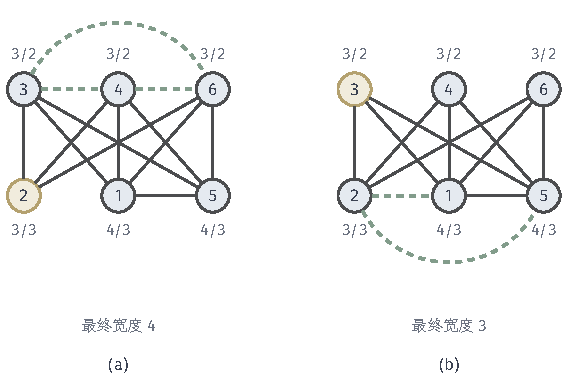
\includegraphics[width=96.778mm]{figures/01-basic-mathematics/04-graphs/tikz/c5-min-degree-min-fill/figure.pdf}
  \caption{最小度规则与最小填充规则的第一步。每个顶点旁的“$d/f$”是当前度数与当前缺边数。左：最小度规则在度数为$3$的顶点中按编号选$2$（黄色），要补三条绿色虚线，最终宽度为$4$。右：最小填充规则选缺边最少的$3$（黄色），只补两条边，最终宽度为$3$。}
  \label{fig:graph-dp-min-degree-min-fill}
\end{figure}

\subsubsection{贪心规则的分析}

\paragraph{启发式的局限}
两种规则都只看一步：度数小不代表补边少，补边少也不保证以后的袋小。上例中最小度规则受平局规则影响，第一步补的三条边把剩余图变成了完全图，得到的宽度比最小填充多$1$。穷举全部$720$个消元次序可以核对，这个图上任何次序的诱导宽度都不小于$3$，所以最小填充在这里恰好达到了最好的次序。换一个图，最小填充同样可能不是最优。因此报告结果时应分开写出构造的宽度、填充边数和结构操作次数，并把宽度理解为树宽的上界，而不是树宽本身。

宽度按变量个数计，而表的项数按状态数之积计。各变量状态数不同时，诱导宽度相同的两个次序，其最大消元簇的配置数可以相差很多；这时可以把评分换成消元簇上的状态数之积，或者构造后直接比较各簇的实际配置数。第~\ref{sec:graph-dp-table-size}小节按实际乘积比较候选结构。

\paragraph{复杂度}
直接实现时每轮要为全部剩余顶点重算评分。最小度规则的评分只需读出度数；最小填充规则要检查每个顶点的每对邻居是否相邻，一轮的检查量可达$\sum_v|N(v)|^2$。用缓存时只重算受影响的顶点：加入边$\{a,b\}$只改变$a$、$b$及其公共邻居的评分，删去$v$只改变$v$的邻居的评分。

\subsection{弦图与完美消元序}
\label{sec:graph-dp-chordal}

填充边会使袋变大，最理想的情形是全程不需要补边。处理顶点$v$时不需要补边，当且仅当$v$的当前邻居已经两两相邻。当前邻居构成团的顶点称为\term{单纯顶点}（simplicial vertex）；没有邻居或只有一个邻居的顶点也算单纯顶点。若一个消元次序使每个顶点在被处理时都是当前图中的单纯顶点，就称它为\term{完美消元序}（perfect elimination ordering）。沿完美消元序消元不产生任何填充边，当前图始终是原图在剩余顶点上的诱导子图。

\paragraph{弦图}
不是每个图都有完美消元序。四个顶点的环$1-2-3-4-1$中，每个顶点的两个邻居都不相邻：$1$与$3$的邻居都是$\{2,4\}$，缺边$\{2,4\}$；$2$与$4$的邻居都是$\{1,3\}$，缺边$\{1,3\}$。所以第一步就找不到单纯顶点。补入边$\{1,3\}$后，顶点$2$的邻居$\{1,3\}$相邻，可以先消去；剩下的三角形$1,3,4$中每个顶点都单纯，于是$(2,1,3,4)$是完美消元序。图~\ref{fig:graph-dp-chordal-four-cycle}画出了这一对比。

\begin{figure}[!htb]
  \centering
  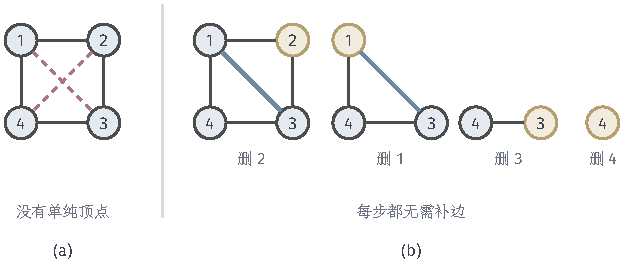
\includegraphics[width=106.306mm]{figures/01-basic-mathematics/04-graphs/tikz/c5-chordal-four-cycle/figure.pdf}
  \caption{无弦四环与补弦后的图。左：四环中每个顶点的两个邻居都不相邻（红色虚线为所缺的边），没有单纯顶点。右：补入弦$\{1,3\}$（蓝色）后，按$(2,1,3,4)$逐个删除，每一步被删除的黄色顶点的剩余邻居都已相邻，全程无填充。}
  \label{fig:graph-dp-chordal-four-cycle}
\end{figure}

四环的问题出在“长度至少为四而没有捷径的环”。消去这种环上的任何一个顶点，它在环上的两个邻居都不相邻，必须补一条边把它们直接连起来；三角形则没有这个问题，因为两个邻居本来就相邻。在长度至少为$4$的环上，连接两个在环上不相邻的顶点的边称为该环的\term{弦}（chord），也就是一条捷径。每个长度至少为$4$的环都有弦的有限无向图称为\term{弦图}（chordal graph）。

树没有环，是弦图；补入$\{1,3\}$后的四环是弦图；无弦四环不是。给一般图补边使之成为弦图称为\term{弦化}（chordal completion）。

\begin{theorem}[弦图与完美消元序]
\label{thm:graph-dp-chordal-peo}
有限无向图是弦图，当且仅当它有完美消元序。
\end{theorem}

\begin{proof}
先证有完美消元序的图是弦图。设图中有长度至少为$4$且无弦的环，考察环上最先被处理的顶点$v$。$v$在环上的两个邻居$u,w$此时都还在图中，并且与$v$相邻。$v$是单纯顶点，所以$u,w$相邻；而沿完美消元序处理时从不补边，$\{u,w\}$必是原图的边。环长至少为$4$，$u,w$在环上不相邻，于是$\{u,w\}$是这个环的弦，矛盾。

反方向的论证路线如下。第一步是一个引理：每个非空有限弦图都有单纯顶点，若它不是完全图，还有两个不相邻的单纯顶点。这一步需要分析极小分隔集，证明极小分隔集在弦图中都是团，本书不展开。第二步，弦图的诱导子图仍是弦图，因为诱导子图中的无弦环在原图中也无弦。于是可以反复删去一个单纯顶点，余下的图仍是弦图、仍有单纯顶点，直到删完，删除的次序就是完美消元序。
\end{proof}

\paragraph{填充图与弦化}
一般图经一次完整消元得到的填充图$\mathcal G^+_\pi$（第~\ref{sec:graph-dp-fill-in}小节）总是弦图，并且$\pi$就是它的完美消元序。要验证这一点，只需说明在$\mathcal G^+_\pi$中，$v$排在它之后的邻居恰是消元时的剩余邻居$N^+_\pi(v)$：$\mathcal G^+_\pi$中连接$v$与某个较晚顶点$w$的边，若是原始边，处理$v$时仍在；若是填充边，它在处理某个更早的顶点时补入，那时$v$还没有被删去，所以处理$v$时这条边也在。于是这些后续邻居在处理$v$时已被补成团，$v$在$\mathcal G^+_\pi$中按$\pi$处理时总是单纯顶点。由定理~\ref{thm:graph-dp-chordal-peo}，$\mathcal G^+_\pi$是弦图，第~\ref{sec:graph-dp-order-to-decomposition}小节的构造实际上隐含了一次弦化。

反过来，设$\mathcal H$是包含$\mathcal G$的弦图（顶点相同、边更多），$\sigma$是$\mathcal H$的完美消元序。按$\sigma$对$\mathcal G$消元，对步数归纳可知当前图始终是$\mathcal H$在剩余顶点上的诱导子图的子图：处理$v$时，它的当前邻居包含在$\mathcal H$中$v$的后续邻居里，后者在$\mathcal H$中成团，所以补入的填充边都是$\mathcal H$的边。因此$\mathcal G^+_\sigma\subseteq\mathcal H$，每个消元簇都含于$\mathcal H$的某个团，诱导宽度不超过$\mathcal H$的最大团大小减一。

这样，消元次序与弦化相互对应：选一个次序就选定了一个弦化，选一个弦化及其完美消元序也就得到一个宽度不更大的次序。四环算例按$(1,2,3,4)$消元，填充图是环加上弦$\{2,4\}$，$(1,2,3,4)$正是它的完美消元序；按$(2,1,3,4)$消元则对应图~\ref{fig:graph-dp-chordal-four-cycle}中补弦$\{1,3\}$的弦化。

\subsection{完美消元序的构造与核验}
\label{sec:graph-dp-peo-construction}

\subsubsection{问题与思路}

定理~\ref{thm:graph-dp-chordal-peo}只说明弦图有完美消元序，没有给出求法。输入是一个有限无向图，输出是它的一个完美消元序，或者“不是弦图”的报告及证据。定理证明的反方向已经提示了做法：反复找一个单纯顶点删去。弦图的每个诱导子图仍有单纯顶点，所以对弦图这一过程不会卡住；非弦图没有完美消元序，过程必然在某一轮找不到单纯顶点，这时剩下的图本身就是证据。

\subsubsection{算法实现}

输入图在运行中不变。算法维护两项状态：
\begin{itemize}
  \item 当前图：初值为输入图的副本；
  \item 已输出的次序：初值为空。
\end{itemize}
每一轮依次做两件事：
\begin{itemize}
  \item 检查：按编号逐个检查当前图中的顶点，枚举它的每对邻居看是否相邻，遇到第一个单纯顶点就停下；
  \item 删除：把找到的单纯顶点从当前图中删去，追加到次序末尾。
\end{itemize}
当前图为空时停止，输出的次序就是完美消元序。若非空的当前图中找不到单纯顶点，就停止并报告输入不是弦图，返回这个当前图作为证据，而不暗中补边。

\begin{algorithm}[逐次删除单纯顶点]
\label{alg:graph-dp-peo-construction}
输入：有限无向图。输出：完美消元序，或“不是弦图”的报告及当前图。
\begin{enumerate}
  \item 令当前图为输入图的副本，次序为空。
  \item 若当前图为空，输出次序并停止。
  \item 按编号检查当前图的顶点，找出第一个邻居两两相邻的顶点$v$；若不存在，报告输入不是弦图，返回当前图并停止。
  \item 从当前图中删去$v$，把$v$追加到次序末尾，回到第2步。
\end{enumerate}
\end{algorithm}

\paragraph{执行过程}
在补弦后的四环上（边$\{1,2\},\allowbreak\{2,3\},\allowbreak\{3,4\},\allowbreak\{1,4\},\allowbreak\{1,3\}$）：
\begin{itemize}
  \item 第$1$轮：顶点$1$的邻居$\{2,3,4\}$缺边$\{2,4\}$，跳过；顶点$2$的邻居$\{1,3\}$相邻，选中并删去。
  \item 第$2$轮：剩下三角形$1,3,4$，顶点$1$的邻居$\{3,4\}$相邻，选中。
  \item 第$3$、$4$轮：依次选中$3$与$4$。
\end{itemize}
输出$(2,1,3,4)$。在无弦四环上，第$1$轮四个顶点都不单纯，过程失败并返回整个四环。

\subsubsection{算法分析}

\paragraph{正确性}
成功时，每个顶点在被删去时都是当前图的单纯顶点，而删点不补边，当前图始终是输入图的诱导子图，所以输出的次序是完美消元序。对弦图，由定理~\ref{thm:graph-dp-chordal-peo}证明中的引理与诱导子图的封闭性，每一轮的当前图都有单纯顶点，过程不会中途失败；对非弦图，若过程成功就得到一个完美消元序，与定理矛盾，所以必然在某一轮失败。

\paragraph{复杂度}
直接实现每轮最多检查$n$个顶点，检查顶点$v$需要$O(|N(v)|^2)$次查边，总检查量最坏可达$O(n^4)$。存在线性时间的专门算法，这里不展开。

\subsubsection{完美消元序的核验}

构造得到的次序应当独立核验，来自别处的次序更应如此。给定原图和一个次序，按下面的步骤检查：
\begin{itemize}
  \item 确认次序恰好包含每个顶点一次，并为每个顶点记下次序位置；
  \item 对每个$v$取出原图中排在它之后的邻居，检查它们是否两两相邻。
\end{itemize}
全部通过时次序是完美消元序，因为在不补边的前提下，处理$v$时的当前邻居恰好就是这些后续邻居；发现缺边时，就把$v$和那对不相邻的邻居作为失败证据返回。例如把$(2,1,3,4)$用于无弦四环，第一个顶点$2$的后续邻居$\{1,3\}$不相邻，立即被拒绝；用于补弦后的图则通过。

核验只需$O(n+m)$再加$\sum_v|N^+_\pi(v)|^2$次查边，比构造便宜得多，所以即使次序来自别处，也值得先核验再使用。

\subsection{团树的构造}
\label{sec:graph-dp-clique-tree}

\subsubsection{问题与思路}

弦图上可以直接用团作袋，这需要区分两种“最大”。不能再加入任何其他顶点而保持两两相邻的团称为\term{极大团}（maximal clique），这是按集合包含判断的；在所有团中顶点数最多的称为\term{最大团}（maximum clique）。例如三角形$1,2,3$外加一条边$\{3,4\}$，极大团是$\{1,2,3\}$和$\{3,4\}$；后者不能再扩大，但只有两个顶点，不是最大团。以弦图的全部极大团为袋、并满足运行交集的树分解称为\term{团树}（junction tree，也称clique tree）。团树中每个袋都是团，没有因填充而多出的变量，相邻两袋的交集就是它们共享的变量。

给定一个弦图，构造团树要做两件事：得到全部极大团，再把它们连成满足运行交集的树。极大团可以从完美消元序中读出。设$\pi$是完美消元序，候选集合$K_v=\{v\}\cup N^+_\pi(v)$就是第~\ref{sec:graph-dp-order-to-decomposition}小节构造中的袋；$v$被处理时是单纯顶点，所以$K_v$是团，极大团就藏在这些候选中。

连接时要选一棵树，使每个变量所在的团连成一片。可以按变量数边：一个变量属于$r$个团时，树中两端都含它的边至多有$r-1$条，再多就会在这$r$个团之间成环；恰有$r-1$条时，这$r$个团才连成一片。反过来看一条树边$\{C,D\}$，它为$C\cap D$中的每个变量各计一条，所以它的贡献是$|C\cap D|$。以交集大小为边权，一棵生成树的总权就等于各变量的这种边数之和，不超过各变量的$r-1$之和；达到这个上限，恰好意味着每个变量的团都连成了一片。这样，连接团的问题变成了最大权生成树问题。把每条边的权取负，就可以直接调用第~\ref{chap:minimum-spanning-tree}章的最小生成树算法，那里的割性质保证Kruskal与Prim方法给出最优树。

\subsubsection{算法实现}

输入是弦图$\mathcal H$，先用第~\ref{sec:graph-dp-peo-construction}小节的方法求出并核验它的完美消元序$\pi$；此后$\mathcal H$与$\pi$都不再改变。算法维护三项状态：
\begin{itemize}
  \item 团表：初值为全部候选$K_v$，处理后只剩极大团；
  \item 候选边表：团两两之间的边及其权$w(C,D)=|C\cap D|$，按权从大到小排列；
  \item 并查集与已选树边：并查集初值为每个团各成一组，已选树边初值为空。
\end{itemize}
计算分三步：
\begin{itemize}
  \item 求极大团：对每个顶点生成候选$K_v$，删去重复的集合和被其他候选严格包含的集合，剩下的就是全部极大团。
  \item 连接：在以极大团为顶点的完全图上，按权从大到小考察候选边，两端不在同一组时加入树边并合并两组，否则跳过；这正是把权取负后调用Kruskal方法：负权的最小生成树就是原权的最大权生成树。也可以改用Prim方法。
  \item 核验：对输出的树逐个顶点检查运行交集。
\end{itemize}
已选树边达到团数减一时，连接停止。

\begin{algorithm}[由弦图构造团树]
\label{alg:graph-dp-clique-tree}
输入：有限弦图$\mathcal H$。输出：$\mathcal H$的团树。
\begin{enumerate}
  \item 求完美消元序$\pi$并核验；对每个顶点$v$生成候选$K_v=\{v\}\cup N^+_\pi(v)$。
  \item 删去重复的候选和被其他候选严格包含的候选，得到极大团$\mathcal C$。
  \item 对$\mathcal C$中每对团计算$w(C,D)=|C\cap D|$，按权从大到小考察，用并查集判断是否成环，不成环时加入树边，直到树边数为$|\mathcal C|-1$。
  \item 对每个顶点检查含它的团在树中是否连通。
\end{enumerate}
\end{algorithm}

\paragraph{执行过程}
图~\ref{fig:graph-dp-clique-tree-mst}的弦图有边$\{1,2\},\allowbreak\{1,3\},\allowbreak\{2,3\},\allowbreak\{2,4\},\allowbreak\{3,4\},\allowbreak\{3,5\},\allowbreak\{4,5\}$。
\begin{itemize}
  \item 完美消元序：取$(1,2,5,3,4)$并核验，各顶点在次序中靠后的邻居分别为$\{2,3\}$、$\{3,4\}$、$\{3,4\}$、$\{4\}$、$\varnothing$，都两两相邻。
  \item 求极大团：候选为$K_1=\{1,2,3\}$、$K_2=\{2,3,4\}$、$K_5=\{3,4,5\}$、$K_3=\{3,4\}$、$K_4=\{4\}$；$K_3$被$K_2$包含，$K_4$被$K_3$包含，删去后得到三个极大团$A=\{1,2,3\}$、$B=\{2,3,4\}$、$C=\{3,4,5\}$。
  \item 计算权：$w(A,B)=|\{2,3\}|=2$、$w(B,C)=|\{3,4\}|=2$、$w(A,C)=|\{3\}|=1$。
  \item 连接：先加入$A-B$，再加入$B-C$，此时三个团已连通，$A-C$会成环而被跳过。得到的最大权生成树是$A-B-C$，总权为$4$。
  \item 核验：含$3$的团$A,B,C$沿$A-B-C$连通，含$2$的团$A,B$相邻，含$4$的团$B,C$相邻，运行交集成立。
\end{itemize}
若改选$A-B$与$A-C$，总权为$3$，此时含$4$的两个团$B,C$之间隔着不含$4$的$A$，运行交集被破坏，如图~\ref{fig:graph-dp-clique-tree-mst}右侧所示。

\begin{figure}[!htb]
  \centering
  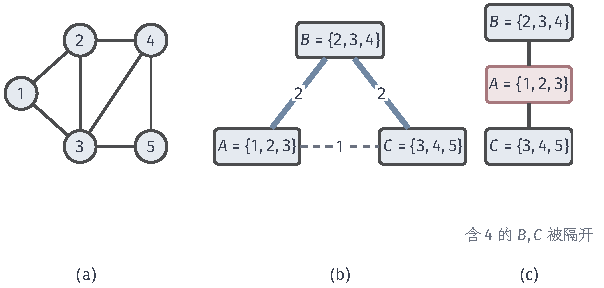
\includegraphics[width=102.306mm]{figures/01-basic-mathematics/04-graphs/tikz/c5-clique-tree-mst/figure.pdf}
  \caption{用交集权重的最大权生成树连接极大团。左：弦图。中：三个极大团组成的候选完全图，边上的数是交集大小，蓝色粗线是总权为$4$的最大权生成树$A-B-C$，虚线是未被选中的候选边。右：总权为$3$的另一棵生成树$B-A-C$，含$4$的团$B,C$被不含$4$的$A$（红色）隔开，不满足运行交集。}
  \label{fig:graph-dp-clique-tree-mst}
\end{figure}

\subsubsection{算法分析}

\paragraph{正确性}
先说明候选集合给出全部极大团。每个$K_v$都是团。反过来，任一团$C$都包含在某个$K_v$中：取$C$中最先被处理的顶点$v$，$C$的其余顶点都在$v$之后且与$v$相邻；沿完美消元序消元不补边也不删去尚未处理的顶点之间的边，它们在处理$v$时仍是$v$的当前邻居，所以都属于$N^+_\pi(v)$。因此每个极大团都等于某个$K_v$（它包含于某个团$K_v$，又是极大的），而不被其他候选严格包含的候选都是极大团。这也说明弦图的极大团数不超过顶点数$n$。

上面的例子中，满足运行交集的树恰好是总权最大的树。下面的定理把思路中的计数写成证明，说明这一对应是一般的。

\begin{theorem}[团树与最大权生成树]
\label{thm:graph-dp-clique-tree-mst}
设$\mathcal H$是非空有限弦图，$\mathcal C$是它的全部极大团。在以$\mathcal C$为顶点的完全图上令$w(C,D)=|C\cap D|$。则一棵生成树满足运行交集，当且仅当它的总权最大。
\end{theorem}

\begin{proof}
先给出任意生成树的总权上界。对生成树$\mathcal T'$，把每条边的权按共享变量拆开计数：
\[
\sum_{\{C,D\}\in\mathcal T'}|C\cap D|=\sum_{v}e_v,
\]
其中$e_v$是两端都含$v$的树边条数。设$v$属于$r_v$个极大团，两端都含$v$的树边正是$\mathcal T'$在这$r_v$个节点上的诱导子图的边；树的诱导子图没有环，是$r_v$个节点上的森林，所以$e_v\leq r_v-1$，且等号成立当且仅当这个诱导子图连通，即含$v$的团在$\mathcal T'$中连通。于是总权不超过$\sum_v(r_v-1)$，等号成立当且仅当对每个$v$都满足运行交集。

剩下要证明确实存在满足运行交集的生成树，即团树存在；那时最大总权恰为$\sum_v(r_v-1)$，最大权生成树就是满足运行交集的生成树。取一个完美消元序，按定理~\ref{thm:graph-dp-elimination-decomposition}的方法以$K_v$为袋得到树分解。若某个袋包含于相邻的袋，就把这条袋树边收缩，只保留较大的袋：顶点覆盖和边覆盖不受影响；对运行交集，被收缩的较小袋中的变量都在较大袋中，收缩一条两端都含$v$的边不破坏$T_v$的连通性，而不含$v$的较小袋本来不在$T_v$中，收缩后$T_v$也不变。

反复收缩，直到没有相邻两袋有包含关系。这时任何两个袋都没有包含关系：若$B_s\subseteq B_t$而$s,t$不相邻，取路径上与$s$相邻的节点$s'$，由运行交集$B_s$的每个变量都在$B_{s'}$中，与“相邻袋无包含关系”矛盾。各袋都是团且互不包含；每个极大团都被某个袋容纳（引理~\ref{lem:graph-dp-clique-in-bag}），而袋本身是团，所以二者相等；每个袋也都是某个极大团，否则它会被那个极大团所在的另一个袋严格包含。于是剩下的袋恰好是全部极大团，各出现一次，团树存在。
\end{proof}

在上例中，$r_1=1$、$r_2=2$、$r_3=3$、$r_4=2$、$r_5=1$，上界$\sum_v(r_v-1)=4$，正好等于$A-B-C$的总权。不连通的弦图中，不同分量的团之间交集为空，零权边只用于把各分量的团树连成一棵树，不影响上界。上面的计数也给出了最后一步核验的做法：检查每个$e_v$是否等于$r_v-1$。

\paragraph{复杂度}
设极大团有$p\leq n$个，候选完全图有$p(p-1)/2$条边，每条边的权需要一次集合求交，排序与并查集的开销按第~\ref{chap:minimum-spanning-tree}章的分析计算。求完美消元序和候选集合的开销见第~\ref{sec:graph-dp-peo-construction}小节与第~\ref{sec:graph-dp-order-to-decomposition}小节。

\paragraph{适用范围}
定理要求输入是弦图，并且使用全部极大团。对无弦四环，极大团是四条边$\{1,2\},\allowbreak\{2,3\},\allowbreak\{3,4\},\allowbreak\{1,4\}$，每个顶点属于两个团；要让每个顶点的两个团相邻，需要四条树边，而四个节点的树只有三条边，所以任何生成树都不满足运行交集。一般图应先弦化，例如用某个消元次序补边，再在弦化后的图上构造团树；在原图的极大团上任选一棵树并不能保证得到树分解。选哪一种弦化决定了袋的大小，而团树构造只负责连接给定弦图的团，不负责找最好的弦化。输出后逐个顶点检查运行交集，也是对输入是否为弦图、团列表是否完整的独立核对。

\subsection{构建结果的检验}
\label{sec:graph-dp-construction-check}

无论结构来自消元次序、贪心规则还是团树构造，交给下一章计算之前都应独立检验。检验只读输出的袋树，不依赖它是怎样构造出来的，所以同样适用于来自别处的分解。检验的对象是原始图$\mathcal G$（有保留集时是$\mathcal G_R$）、局部函数的作用域、袋树及选定的根。

\paragraph{树分解的三个条件}
核验按定义逐条进行：确认袋树是树，即节点数减一等于边数且连通；扫描各袋得到每个顶点的$T_v$，检查顶点覆盖与边覆盖；对每个顶点$v$数出两端袋都含$v$的袋树边条数$e_v$。这些边恰是树在$T_v$上的诱导子图的边，而树的诱导子图是森林，所以$e_v\leq|T_v|-1$，等号成立当且仅当$T_v$连通。

图~\ref{fig:graph-dp-running-intersection}下面的连接中$|T_2|=2$而$e_2=0$，核验失败，$2$就是失败的证据；梯子的分解中$|T_2|=3$、$e_2=2$，通过。团树构造中的最后一步核验（检查每个$e_v$是否等于$r_v-1$）也是这一检查。

\paragraph{作用域、接口与查询}
树分解的条件只涉及原始图的边。计算还需要每个局部函数有处可放，所以对每个作用域$S_a$找出一个包含它的袋并记录下来；引理~\ref{lem:graph-dp-clique-in-bag}保证合法的分解总能通过这项检查，找不到时说明分解本身有误或作用域与原始图不符。

选定根以后，为每个非根节点算出接口$S_u=B_u\cap B_{p(u)}$与内部变量$I_u$，并核对每个变量恰在一个节点作内部变量（引理~\ref{lem:graph-dp-unique-internal}）。有保留集$R$时，另检查根袋包含$R$。最后记录实际宽度，以及各袋、各接口上的状态数之积，供第~\ref{sec:graph-dp-computation-cost}节估计代价。

\paragraph{检验的代价}
设袋树有$N$个节点，各袋大小之和为$L=\sum_t|B_t|$。建立每个顶点的$T_v$和数出各$e_v$需要扫描各袋及各条袋树边两端的公共变量，时间为$O(L+n)$量级（用以变量为下标的数组标记袋内成员）；边覆盖与作用域容纳的检查对每条边或每个作用域，在最小的$T_v$中逐袋测试包含关系。这些都是关于袋大小的多项式开销，与随状态数指数增长的数值计算相比通常很小，但它们是构建阶段的成本，应与构造本身的成本分开记录，不计入下一章的求值时间。

四环算例的分解$\{1,2,4\}-\{2,3,4\}$以$\{2,3,4\}$为根时，检验结果为：四条边分别被两个袋覆盖；$e_2=e_4=1=|T_2|-1=|T_4|-1$，$e_1=e_3=0=|T_1|-1=|T_3|-1$；四个作用域$\{1,2\},\{1,4\}$放进第一个袋，$\{2,3\},\{3,4\}$放进根袋；子节点的接口为$\{2,4\}$、内部变量为$\{1\}$，根的内部变量为$\{2,3,4\}$；宽度为$2$，每个袋上有$8$种配置，接口上有$4$种。
